\documentclass[12pt]{article}
\usepackage[english]{babel}
\usepackage{natbib}
\usepackage{url}
\usepackage{hyperref}
\usepackage{minted}
\usemintedstyle{borland}
\usepackage{listings}
\usepackage[utf8x]{inputenc}
\usepackage{graphicx}
\graphicspath{{images/}}
\usepackage{fancyhdr}
\usepackage{vmargin}
\setmarginsrb{3 cm}{2.5 cm}{3 cm}{2.5 cm}{1 cm}{1.5 cm}{1 cm}{1.5 cm}
%%%%%%%%%%%%%%%%%%%%%%%%%%%%%%%%%%%%%%%%%%%%%%%%%%%%%%%%%%%%%%%%%%%%%%%%%%%%%%%%%%%%%%%%%
\title{Práctica 4: Round Robin}% Title 
\author{Meza Madrid Damián}% Author
\date{Marzo 2019}% Date
%%%%%%%%%%%%%%%%%%%%%%%%%%%%%%%%%%%%%%%%%%%%%%%%%%%%%%%%%%%%%%%%%%%%%%%%%%%%%%%%%%%%%%%%%
\makeatletter
\let\thetitle\@title
\let\theauthor\@author
\let\thedate\@date
\def\@seccntformat#1{%
\expandafter\ifx\csname c@#1\endcsname\c@section\else
\csname the#1\endcsname\quad
\fi}
\makeatother
\pagestyle{fancy}
\fancyhf{}
\rhead{\theauthor}
\lhead{\thetitle}
\cfoot{\thepage}
\begin{document}

%%%%%%%%%%%%%%%%%%%%%%%%%%%%%%%%%%%%%%%%%%%%%%%%%%%%%%%%%%%%%%%%%%%%%%%%%%%%%%%%%%%%%%%%%

\begin{titlepage}
	\centering
    \vspace*{0.5 cm}
    
\includegraphics[scale = 0.30]{escom.png}\\[1.0 cm]	% University Logo
	\textsc{\Large Instituto Politécnico Nacional}\\[0.5 cm]% Course Code
	\textsc{\Large Escuela Superior de Computo}\\[0.5 cm]% Course Code
	\rule{\linewidth}{0.2 mm} \\[0.4 cm]
	{ \huge \bfseries \thetitle}\\
	\rule{\linewidth}{0.2 mm} \\[1.5 cm]
	Reporte\\
	Profesor: Ulises Velez Saldaña \\
	Alumno: Meza Madrid Raúl Damián\\
    Clase: Sistemas operativos\\
    Grupo: 2CM7\\
\end{titlepage}
\tableofcontents
\pagebreak
\section{Introducción}
Una computadora multiprogramada suele tener varios procesos compitiendo por la CPU al mismo tiempo. Esta situación se presenta cada vez que dos o mas procesos están en el estado listo en forma simultanea. Si solo se cuenta con una CPU, es preciso decidir cual proceso se ejecutará. El sistema se hace cargo de tomar esta decisión haciendo uso de un algoritmos de planificación. 
\subsection{Planificador}
Además de escoger el proceso mas conveniente a ejecutar, el planificador debe preocuparse por aprovechar con eficiencia la CPU, ya que la conmutación de procesos es costosa. En general se puede decir que la meta de el planificador, como el de su respectivo algoritmo, es el de lograr que todas las partes del sistema estén ocupadas; esto quiere decir que el CPU y los dispositivos de entrada y salida (I/O) estén trabajando todo el tiempo para así ganar mayor rendimiento que si algunos de los componentes estuvieran inactivos.\\
El planificador puede ser diseñado de diferentes maneras, para servir a diferentes tipos de procesos y sistemas, atendiendo con prioridades como \emph{primera entrada primera salida } o \emph{Trabajo mas corto primero}. En esta practica nos dedicaremos a uno de los más antiguos, sencillos, equitativos y ampliamente utilizados; el turno circular o round robin.
\subsection{Round-robin}
A cada proceso se le asigna un intervalo de tiempo llamado \emph{cuanto} durante el que se le permitirá ejecutarse. Si al termino del \emph{cuanto}, el proceso se sigue ejecutando, se le expropia la CPU para asignársela a otro proceso. Si un proceso termina antes de expirar su \emph{cuanto}, la conmutación de la CPU se efectúa inmediatamente.\\
La implementación del turno circular es sencillo, lo único que se necesita es mantener una lista de procesos ejecutables como se muestra en la figura\ref{fig:listas}
\begin{figure}
    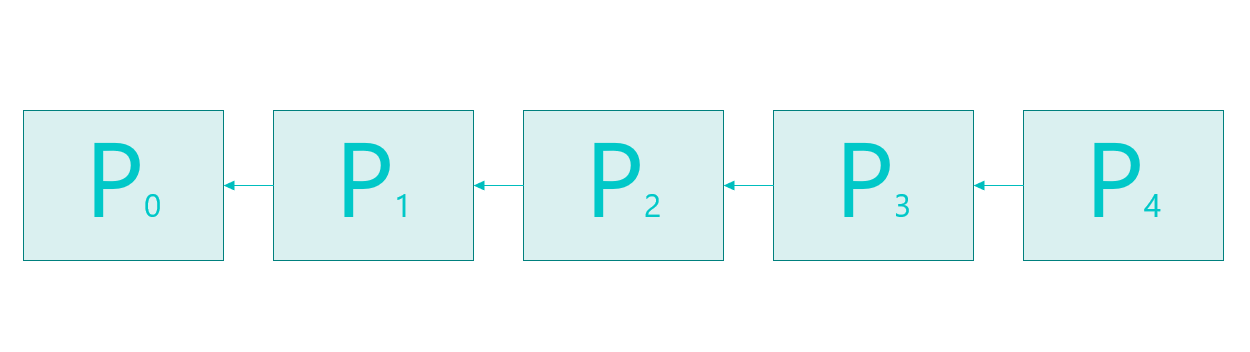
\includegraphics[width=\textwidth]{r-r-0.png}
    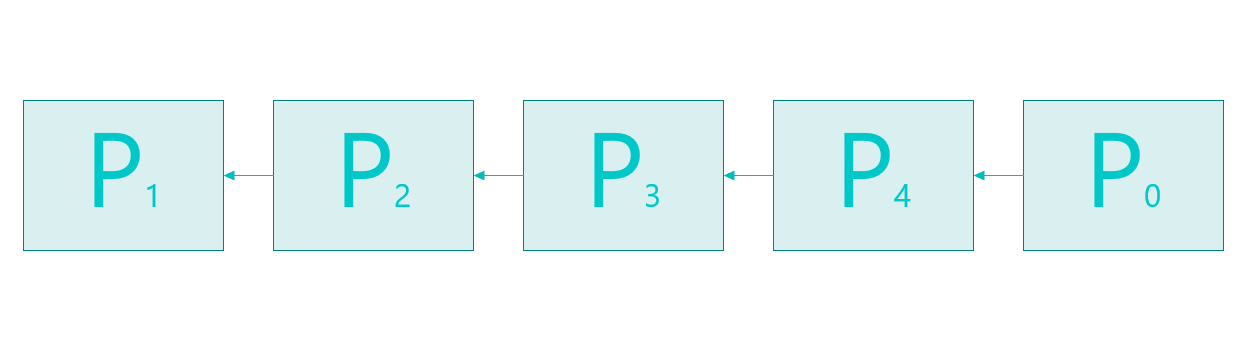
\includegraphics[width=\textwidth]{r-r-1.png}
    \caption{En la parte superior se muestra el estado inicial de la lista de procesos, en la parte inferior se muestra como resulta despues de que el cuanto se agota.}
    \label{fig:listas}
\end{figure}
 Esta es una solución sencilla y equitativa para administrar los proceso donde la única cuestión a considerar es la magnitud del \emph{cuanto}, ya que un cuanto demasiado corto causa demasiadas conmutaciones de procesos y reduce la eficiencia de la CPU, pero uno demasiado corto causa demasiadas conmutaciones de procesos y reduce la eficiencia de la CPU, pero uno demasiado largo puede reducir la rapidez a solicitudes interactivas cortas. Un cuanto al rededor de 20-50 veces el tiempo de conmutación suele ser un tiempo razonable.
\subsection{Programas y herramientas utilizados}
Esta práctica fue desarrollada en el sistema operativo Ubuntu 18.04.1 LTS. Estos son los programas y herramientas utilizados, junto con el comando de instalación, en caso de que no estuvieran instalados ya. 
\begin{itemize}
    \item Doxygen 
    \begin{minted}{bash}
        git clone https://github.com/doxygen/doxygen.git
        cd doxygen
        mkdir build
        cd build
        cmake -G "Unix Makefiles" ..
        make
        make install
    \end{minted}
    \item make
    \item cmake
    \item python
\end{itemize}
\section{Objetivo}
Que el alumno aplique la teoría vista en clase, visualizando el algoritmo de planificación \emph{Round-Robin}
\section{Desarrollo}
Para simular el funcionamiento del Round Robin se necesita usar una cola circular, para simular la llegada de los procesos se usara una cola y finalmente se usara una clase proceso para almacenar la información de cada proceso como su duración, su llegada y su id. Cada clase contendrá su método \_\_str\_\_ para facilitar la visualización en terminal.\cite{str}
\subsection{Cola Circular}
La cola circular se puede ver como una lista simplemente ligada mas dos apuntadores o variables que apuntan al inicio y al fin de la cola.\\
Primero se crearan los nodos para la lista simplemente ligada
\subsubsection{Código fuente: Nodo}
\begin{minted}[breaklines,mathescape, linenos, numbersep=5pt, frame=single, numbersep=5pt, xleftmargin=0pt]{python}
## Estructura base para la cola circular
class node:
    ##Constructor
    #@param self apuntador al objeto
    #@param val valor del nodo
    #@param next apuntador al siguiente elemento
    def __init__(self, val,next):
        ##valor del nodo
        self.value = val
        ## apuntador al siguiente elemento
        self.next = next
    ##Modifica el apuntador al siguiente objeto
    def sNext(self, next):
        self.next = next
    ##Regresa el elemento siguiente del objeto
    def gNext(self,next):
        return self.next

\end{minted}
Ya teniendo los nodos como base para la cola circular, solo es necesario mantener seguimiento del frente y fin de la cola, así como los métodos para insertar elementos, quitar elementos  y rotar la cola
\subsubsection{Código fuente: Cola Circular}
\begin{minted}[breaklines,mathescape, linenos, numbersep=5pt, frame=single, numbersep=5pt, xleftmargin=0pt]{python}
from node import node
## Cola circular, utiliza node como base para hacer una lista simplemente ligada
class CircularQ:
    ##Constructor, crea dos variables que apuntan al frente y fin de la cola
    def __init__(self):
        ##Frente de la cola
        self.front = None
        ##Frente de la cola
        self.rear = None

    ## Crea un nodo y lo agrega a la cola
    #@param self apuntador a objeto
    #@param val valor a agregar en la cola
    def queue(self,val):
        t = node(val,self.front)
        if self.front ==  None:
            self.front = t
            self.front.sNext(self.front)
            self.rear = self.front
        elif(self.rear == self.front):
            self.front.next = t
            self.rear = t
        else:
            self.rear.sNext(t)
            self.rear = t

    ## Quita el nodo 'front' de la cola
    #@param self apuntador a objeto
    def dequeue(self):
        if self.front == self.rear:
            self.front=None
            self.rear=None
            return
        res = self.front
        self.front = self.front.next
        self.rear.sNext(self.front)
        return self.front

    ## Mueve los apuntadores de frente y fin de la cola para que el frente sea el nuevo fin y el segundo elemento sea el nuevo frent
    #@param self apuntador a objeto
    def rotate(self):
        if self.front != self.rear:
            self.rear= self.front
            self.front = self.front.next

    ## Representacion en cadena del objeto
    #@param self apuntador a objeto
    def __str__(self):
        if self.front == None:
            return '||'
        res = str(self.front.value) + '->'
        currNode = self.front.next
        while currNode != self.front:
            res+=str(currNode.value)+'->'
            currNode = currNode.next
        return (res +'/')

\end{minted}
\subsection{Round-Robin}
El programa para simular el round robin se encarga de leer la entrada desde un archivo de texto con el siguiente contenido
en la primer linea se encuentra el numero entero n que equivale al chunck size o cuanto, en las lineas consecutivas se encuentran los las lineas con \[i_k \;\;\;j_k\]separados por un espacio donde  i es el inicio del k-ésimo proceso y j es la duración del mismo, donde\[i_{k}<i_{k+1}\] 
Cada proceso es guardado dentro de una cola o lista simplemente ligada 
\subsubsection{Código fuente: Cola}
\begin{minted}[breaklines,mathescape, linenos, numbersep=5pt, frame=single, numbersep=5pt, xleftmargin=0pt]{python}
## Implementacion de una cola simplemente ligada.
class Queue:
    ##Constructor
    #@param self apuntador al objeto
    def __init__(self):
        ## Contenido del nodo de la lista
        self.head = None
        ## Apuntador al siguiente nodo de la lista
        self.next = None

    ##Metodo para agregar elementos a la lista
    #@param self apuntador al objeto
    #@param val valor del elemento a insertar en la list
    def queue(self,val):
        if self.head == None:
            self.head = val
            self.next = Queue()
        else:
            self.next.queue(val)

    ##Metodo para meter el primer elemento de la lista
    #@param self apuntador al objeto
    def dequeue(self):
        res = self.head
        if self.head != None:
            self.head = self.next.head
            self.next = self.next.next
        return res

    ##Presentacion en cadena de un objeto
    #@param self xapuntador al objeto
    def __str__(self):
        res = ''
        if self.head != None:
            res+=str(self.head) + '->'
            return (res + str(self.next))
        else:
            return ('||')

\end{minted}
Se agrego también la clase proceso para facilitar la los metodos de acceso del mismo
\subsubsection{Código fuente: Proceso}
\begin{minted}[breaklines,mathescape, linenos, numbersep=5pt, frame=single, numbersep=5pt, xleftmargin=0pt]{python}
##Esta clase se encarga de almacenar los datos de cada proceso; id, inicio y duracion, asi como de dar formato a travez del metodo ___str__ para que se pueda usar en print()

class Process:
    ## Variable estatica de la clase para asignar un id unico a cada proceso
    id = 0
    ## Constructor de la clase, se encarga de generar el proceso con id unico tomado de la variable de clase Process.id
    #@param self el apuntador al objeto
    #@param start el ciclo en el que el proceso comenzará
    #@param dur la duracion del proceso antes de terminar.
    def __init__(self,start,dur):
        ## id del proceos
        self.id = Process.id
        Process.id += 1
        ## ciclo en el que llega el proceso al round robin
        self.start = start
        ## duracion del proceso en ciclos
        self.dur = dur
    ## Representacion en cadena de un objeto.
    #@param self el apuntador al objeto
    def __str__(self):
        return '[P'+str(self.id).ljust(2)+'|'+str(self.dur).ljust(2)+']'
\end{minted}
Finalmente el programa se encarga de repetir simular el programa hasta que ambos la cola de procesos pendientes de iniciar y la cola circular de procesos aun no concluidos terminen vacias. 
\subsubsection{Código fuente: Round Robin}
\begin{minted}[breaklines,mathescape, linenos, numbersep=5pt, frame=single, numbersep=5pt, xleftmargin=0pt]{python}
from proc import Process as pr
from circularQ import CircularQ as cq
from queue import Queue as q
from os import system
import time
## brief Programa driverpara la simulacion de round robin
## Cola de procesos que no han entrado al round robin
prcssQ = q()
## Cola circular de round robin
round = cq()
with open('src/input.txt','r') as file:
    file = file.readlines()
    chunkSize = int(file[0])
    for line in file[1:]:
        start, dur = [int(x) for x in line.split()]
        Pn = pr(start, dur)
        prcssQ.queue(Pn)
    cycl = 0
    currP = 0
    while prcssQ.head != None or round.front != None:
        if round.front != None:
            if round.front.value.dur>0:
                round.front.value.dur-=1
            else:
                currP = 0
                round.dequeue()
        system('clear')
        while prcssQ.head != None and prcssQ.head.start == cycl:
            p=prcssQ.dequeue()
            round.queue(p)
        print(''.center(63,'-'))
        print('|'+'Procesos pendientes'.center(40)+'|'+('Ciclo: '+str(cycl)).center(20) + '|')
        print(''.center(63,'-'))
        print('|'+str(prcssQ).center(61)+'|')
        print(''.center(63,'-'))
        print('|'+'Round Robin'.center(61)+'|')
        print(''.center(63,'-'))
        print(round)
        time.sleep(1)
        cycl+=1
        currP+=1
        if currP>chunkSize:
            round.rotate()
            currP=0
    print('End of program')
\end{minted}
\section{Resultados}
El programa muestra el ciclo actual, la lista de procesos que un no han \emph{llegado} y la respectiva cola de procesos ya listos para ser ejecutados. en vez de usar una imagen, se sacaron los resultados a un archivo de texto usando 
\subsection{Caso de prueba: Entrada}
\begin{minted}[breaklines,mathescape, numbersep=5pt,linenos, frame=single, numbersep=5pt, xleftmargin=0pt,]{bash}
1 #Chunk size
#Los primeros dos procesos entran instantaneamente
0 4 #Duracion 4
0 7 #Duracion 7
#El siguiente proceso entra en el ciclo dos 
2 3 #Duracion 3
#El siguiente proceso entra en el ciclo diez
10 6 #Duracion 6
#El siguiente proceso entra en el ciclo trece
13 9 #Duracion 9
\end{minted}
\subsection{Caso de prueba: salida}
\begin{minted}[breaklines,mathescape, numbersep=5pt,linenos, frame=single, numbersep=5pt, xleftmargin=0pt,]{bash}
---------------------------------------------------------------
|          Procesos pendientes           |      Ciclo: 0      |
---------------------------------------------------------------
|          [P0 |12]->[P1 |3 ]->[P2 |1 ]->[P3 |10]->||         |
---------------------------------------------------------------
|                         Round Robin                         |
---------------------------------------------------------------
||
---------------------------------------------------------------
|          Procesos pendientes           |      Ciclo: 1      |
---------------------------------------------------------------
|               [P1 |3 ]->[P2 |1 ]->[P3 |10]->||              |
---------------------------------------------------------------
|                         Round Robin                         |
---------------------------------------------------------------
[P0 |11]->/
---------------------------------------------------------------
|          Procesos pendientes           |      Ciclo: 2      |
---------------------------------------------------------------
|                    [P2 |1 ]->[P3 |10]->||                   |
---------------------------------------------------------------
|                         Round Robin                         |
---------------------------------------------------------------
[P0 |10]->[P1 |3 ]->/
---------------------------------------------------------------
|          Procesos pendientes           |      Ciclo: 3      |
---------------------------------------------------------------
|                    [P2 |1 ]->[P3 |10]->||                   |
---------------------------------------------------------------
|                         Round Robin                         |
---------------------------------------------------------------
[P0 |9 ]->[P1 |3 ]->/
---------------------------------------------------------------
|          Procesos pendientes           |      Ciclo: 4      |
---------------------------------------------------------------
|                         [P3 |10]->||                        |
---------------------------------------------------------------
|                         Round Robin                         |
---------------------------------------------------------------
[P0 |8 ]->[P1 |3 ]->[P2 |1 ]->/
---------------------------------------------------------------
|          Procesos pendientes           |      Ciclo: 5      |
---------------------------------------------------------------
|                         [P3 |10]->||                        |
---------------------------------------------------------------
|                         Round Robin                         |
---------------------------------------------------------------
[P0 |7 ]->[P1 |3 ]->[P2 |1 ]->/
---------------------------------------------------------------
|          Procesos pendientes           |      Ciclo: 6      |
---------------------------------------------------------------
|                         [P3 |10]->||                        |
---------------------------------------------------------------
|                         Round Robin                         |
---------------------------------------------------------------
[P1 |2 ]->[P2 |1 ]->[P0 |7 ]->/
---------------------------------------------------------------
|          Procesos pendientes           |      Ciclo: 7      |
---------------------------------------------------------------
|                         [P3 |10]->||                        |
---------------------------------------------------------------
|                         Round Robin                         |
---------------------------------------------------------------
[P1 |1 ]->[P2 |1 ]->[P0 |7 ]->/
---------------------------------------------------------------
|          Procesos pendientes           |      Ciclo: 8      |
---------------------------------------------------------------
|                         [P3 |10]->||                        |
---------------------------------------------------------------
|                         Round Robin                         |
---------------------------------------------------------------
[P1 |0 ]->[P2 |1 ]->[P0 |7 ]->/
---------------------------------------------------------------
|          Procesos pendientes           |      Ciclo: 9      |
---------------------------------------------------------------
|                         [P3 |10]->||                        |
---------------------------------------------------------------
|                         Round Robin                         |
---------------------------------------------------------------
[P2 |1 ]->[P0 |7 ]->/
---------------------------------------------------------------
|          Procesos pendientes           |     Ciclo: 10      |
---------------------------------------------------------------
|                         [P3 |10]->||                        |
---------------------------------------------------------------
|                         Round Robin                         |
---------------------------------------------------------------
[P2 |0 ]->[P0 |7 ]->/
---------------------------------------------------------------
|          Procesos pendientes           |     Ciclo: 11      |
---------------------------------------------------------------
|                              ||                             |
---------------------------------------------------------------
|                         Round Robin                         |
---------------------------------------------------------------
[P0 |7 ]->[P3 |10]->/
---------------------------------------------------------------
|          Procesos pendientes           |     Ciclo: 12      |
---------------------------------------------------------------
|                              ||                             |
---------------------------------------------------------------
|                         Round Robin                         |
---------------------------------------------------------------
[P0 |6 ]->[P3 |10]->/
---------------------------------------------------------------
|          Procesos pendientes           |     Ciclo: 13      |
---------------------------------------------------------------
|                              ||                             |
---------------------------------------------------------------
|                         Round Robin                         |
---------------------------------------------------------------
[P0 |5 ]->[P3 |10]->/
---------------------------------------------------------------
|          Procesos pendientes           |     Ciclo: 14      |
---------------------------------------------------------------
|                              ||                             |
---------------------------------------------------------------
|                         Round Robin                         |
---------------------------------------------------------------
[P0 |4 ]->[P3 |10]->/
---------------------------------------------------------------
|          Procesos pendientes           |     Ciclo: 15      |
---------------------------------------------------------------
|                              ||                             |
---------------------------------------------------------------
|                         Round Robin                         |
---------------------------------------------------------------
[P0 |3 ]->[P3 |10]->/
---------------------------------------------------------------
|          Procesos pendientes           |     Ciclo: 16      |
---------------------------------------------------------------
|                              ||                             |
---------------------------------------------------------------
|                         Round Robin                         |
---------------------------------------------------------------
[P0 |2 ]->[P3 |10]->/
---------------------------------------------------------------
|          Procesos pendientes           |     Ciclo: 17      |
---------------------------------------------------------------
|                              ||                             |
---------------------------------------------------------------
|                         Round Robin                         |
---------------------------------------------------------------
[P3 |9 ]->[P0 |2 ]->/
---------------------------------------------------------------
|          Procesos pendientes           |     Ciclo: 18      |
---------------------------------------------------------------
|                              ||                             |
---------------------------------------------------------------
|                         Round Robin                         |
---------------------------------------------------------------
[P3 |8 ]->[P0 |2 ]->/
---------------------------------------------------------------
|          Procesos pendientes           |     Ciclo: 19      |
---------------------------------------------------------------
|                              ||                             |
---------------------------------------------------------------
|                         Round Robin                         |
---------------------------------------------------------------
[P3 |7 ]->[P0 |2 ]->/
---------------------------------------------------------------
|          Procesos pendientes           |     Ciclo: 20      |
---------------------------------------------------------------
|                              ||                             |
---------------------------------------------------------------
|                         Round Robin                         |
---------------------------------------------------------------
[P3 |6 ]->[P0 |2 ]->/
---------------------------------------------------------------
|          Procesos pendientes           |     Ciclo: 21      |
---------------------------------------------------------------
|                              ||                             |
---------------------------------------------------------------
|                         Round Robin                         |
---------------------------------------------------------------
[P3 |5 ]->[P0 |2 ]->/
---------------------------------------------------------------
|          Procesos pendientes           |     Ciclo: 22      |
---------------------------------------------------------------
|                              ||                             |
---------------------------------------------------------------
|                         Round Robin                         |
---------------------------------------------------------------
[P3 |4 ]->[P0 |2 ]->/
---------------------------------------------------------------
|          Procesos pendientes           |     Ciclo: 23      |
---------------------------------------------------------------
|                              ||                             |
---------------------------------------------------------------
|                         Round Robin                         |
---------------------------------------------------------------
[P0 |1 ]->[P3 |4 ]->/
---------------------------------------------------------------
|          Procesos pendientes           |     Ciclo: 24      |
---------------------------------------------------------------
|                              ||                             |
---------------------------------------------------------------
|                         Round Robin                         |
---------------------------------------------------------------
[P0 |0 ]->[P3 |4 ]->/
---------------------------------------------------------------
|          Procesos pendientes           |     Ciclo: 25      |
---------------------------------------------------------------
|                              ||                             |
---------------------------------------------------------------
|                         Round Robin                         |
---------------------------------------------------------------
[P3 |4 ]->/
---------------------------------------------------------------
|          Procesos pendientes           |     Ciclo: 26      |
---------------------------------------------------------------
|                              ||                             |
---------------------------------------------------------------
|                         Round Robin                         |
---------------------------------------------------------------
[P3 |3 ]->/
---------------------------------------------------------------
|          Procesos pendientes           |     Ciclo: 27      |
---------------------------------------------------------------
|                              ||                             |
---------------------------------------------------------------
|                         Round Robin                         |
---------------------------------------------------------------
[P3 |2 ]->/
---------------------------------------------------------------
|          Procesos pendientes           |     Ciclo: 28      |
---------------------------------------------------------------
|                              ||                             |
---------------------------------------------------------------
|                         Round Robin                         |
---------------------------------------------------------------
[P3 |1 ]->/
---------------------------------------------------------------
|          Procesos pendientes           |     Ciclo: 29      |
---------------------------------------------------------------
|                              ||                             |
---------------------------------------------------------------
|                         Round Robin                         |
---------------------------------------------------------------
[P3 |0 ]->/
---------------------------------------------------------------
|          Procesos pendientes           |     Ciclo: 30      |
---------------------------------------------------------------
|                              ||                             |
---------------------------------------------------------------
|                         Round Robin                         |
---------------------------------------------------------------
||
\end{minted}
\section{Errores y problemas}

\begin{figure}[!htb]
\begin{minipage}{0.45\textwidth}
Siendo que ahora se usaron diferentes clases para el programa, fue necesario documentarlas con doxygen, pero aunque doxygen no te obliga a documentar cada miembro de las clases, muestra alertas de aquellos que fueron omitidos. 
\end{minipage}
\begin{minipage}{0.45\textwidth}
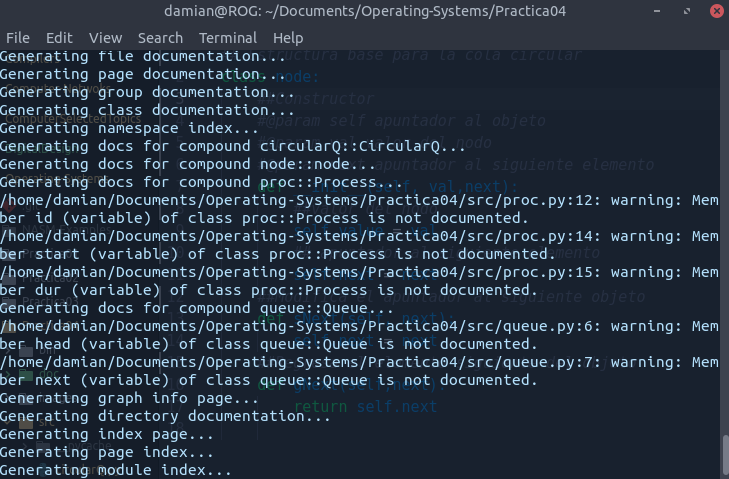
\includegraphics{errors.png}
\end{minipage}
\end{figure}

\begin{figure}[!htb]
\begin{minipage}{0.45\textwidth}
Para resolverlo se fue revisando una por una las lineas de salida en terminal hasta terminar con la siguiente salida
\end{minipage}
\begin{minipage}{0.45\textwidth}
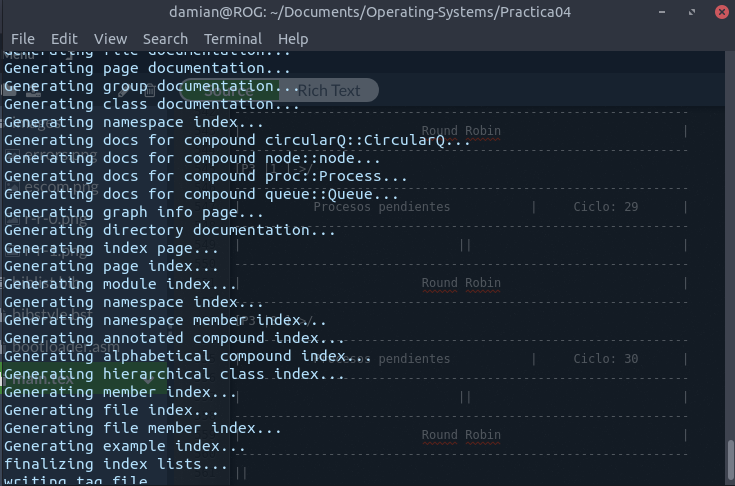
\includegraphics{fix.png}
\end{minipage}
\end{figure}


\section{Codigo (Github)}
Todo el codigo de esta practica se puede encontrar en :\url{https://github.com/asdf1234Damian/Operating-Systems/tree/master/Practica04}
\nocite{*}
\addcontentsline{toc}{section}{References}
\bibliographystyle{plain}
\bibliography{biblist}
\end{document}

